\subsection{Update step}
\label{subsec:toro_update}
The update equation of the EKF is given in Equation \ref{eq:ekf_correct}. The measurement equation of the system is given by $$\hat{y}_{k+1} = h(\hat{x}_{k+1}^-,u_{k+1},0).$$ For the sake of simplicity let us assume the measurement of noise uncorrelated. That is the noise acting on a measurement does not depend on the noise acting on all other measurements. $$V_k = I_3.$$ Substituting the assumption in Equation \ref{eq:ekf_correct} gives
\begin{equation}
\label{eq:correct}
\begin{split}
K_{k+1} &= P_{k+1}^-\hat{C}_{k+1}^{T-}(\hat{C}_{k+1}^-P_{k+1}^-\hat{C}_{k+1}^{T-} + R_{k+1})^{-1}\\
\hat{x}_{k+1} &= \hat{x}_{k+1}^- + K_{k+1}(y_{k+1}-\hat{y}_{k+1})\\
P_{k+1} &= (I- K_{k+1}\hat{C}_{k+1}^-)P_{k+1}^-.
\end{split}
\end{equation}
The measurements of \emph{Toro} are Cartesian accelerations($acc^b$) of the hip measured by accelerometer, angular velocity($\omega^b$) of the hip measured by the gyroscope, joint angles($q_j$) and joint velocities($\dot{q_j}$) measured by joint encoders.
\begin{equation}
    \label{eq:y_sens}
     y_{sens} = \begin{bmatrix} acc^b \\ \omega^b \\ q_j \\ \dot{q}_j \end{bmatrix} 
\end{equation}
\begin{itemize}
    \item The simplified model of $IMU_{acc}$ is $$ acc^b= \begin{bmatrix} acc^b_x \\ acc^b_y \\ acc^b_z \end{bmatrix} =  \begin{bmatrix}\ddot{p}_x^b \\ \ddot{p}_y^b \\ \ddot{p}_z^b \end{bmatrix} - R^T \begin{bmatrix}0 \\0 \\-9.81 \end{bmatrix}$$ \emph{R} is the rotational matrix that transforms a vector in body coordinate frame to spatial frame.
    \item $\ddot{p}^b$ is computed from the forward dynamic equation \ref{eq:motion} using the predicted values of the state
    \item $\omega_{f}^{b} $ is the vector of angular rates of the hip(floating base) measured by gyroscope. The measurements are in the frame attached to the hip. 
\end{itemize}
\begin{figure}
    \begin{center}
    %trim option's parameter order: left bottom right top
    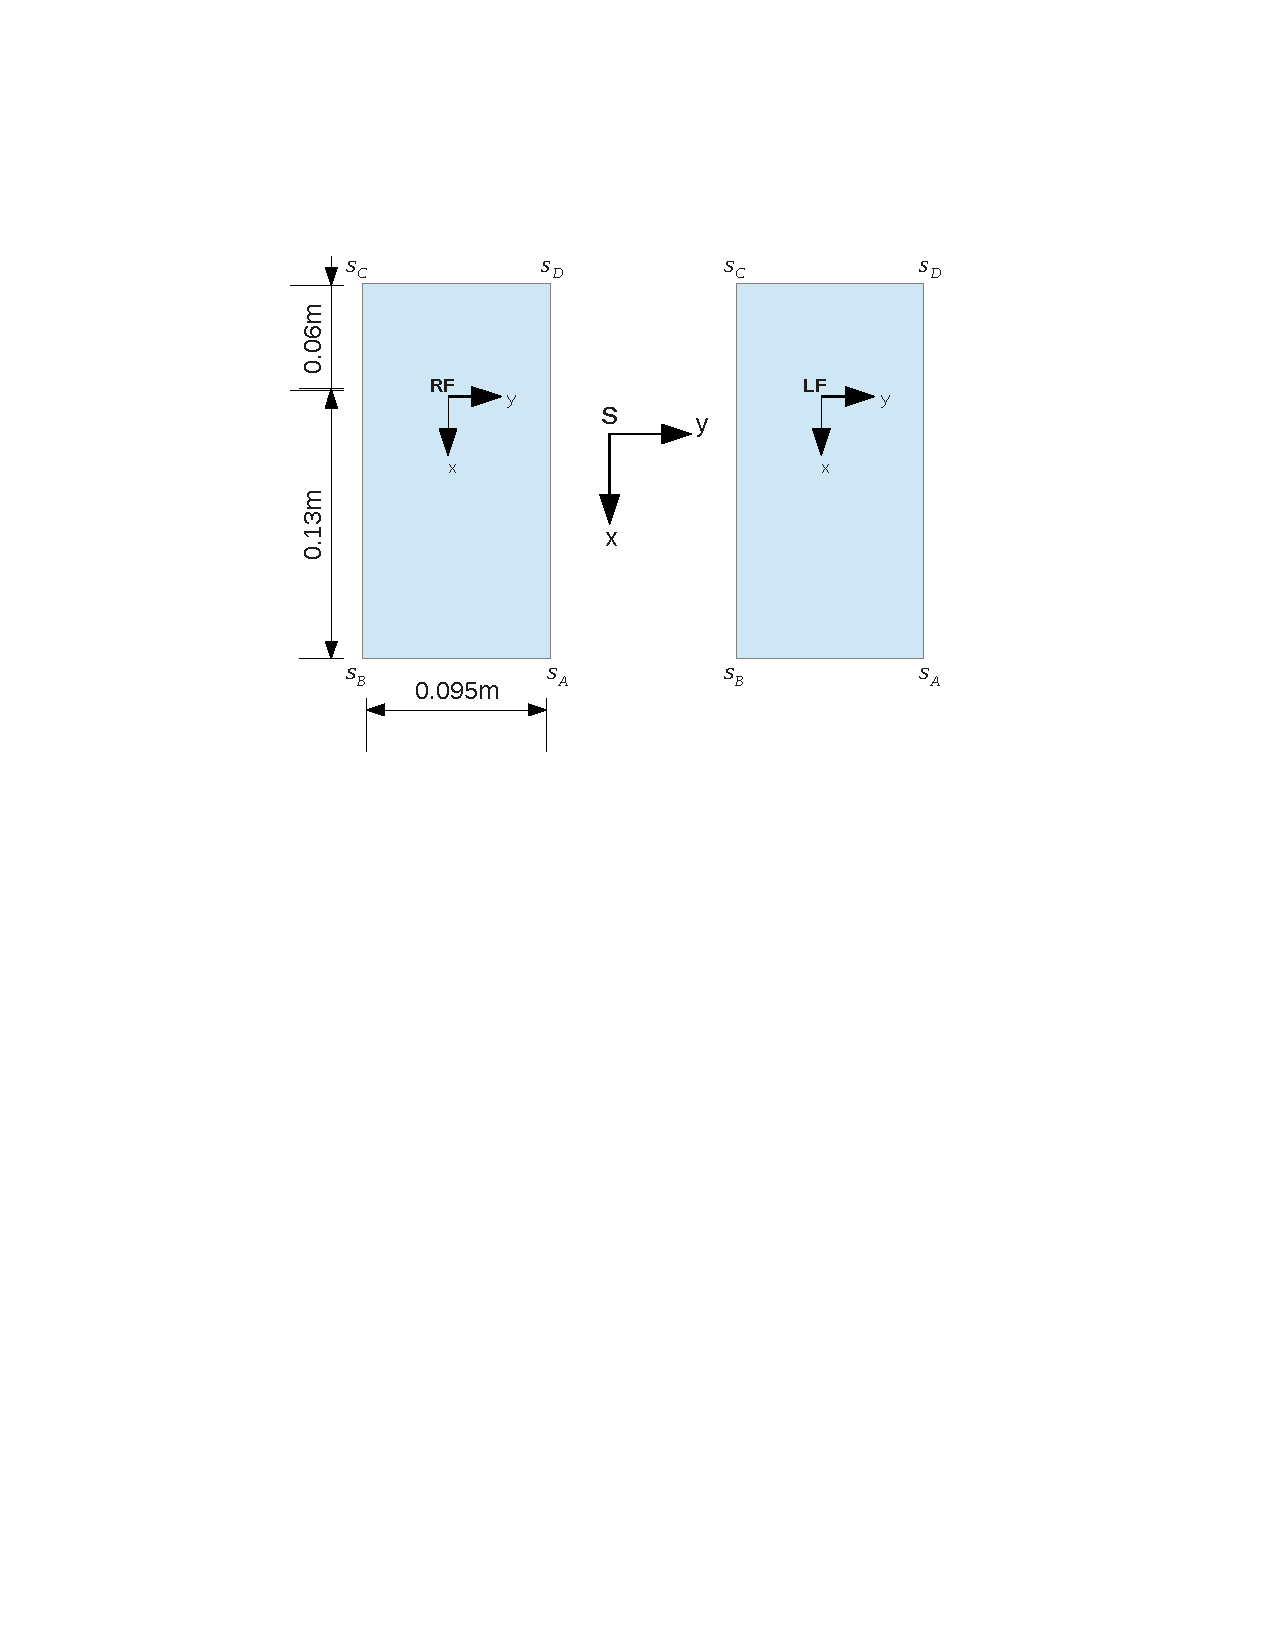
\includegraphics[trim= 20mm 150mm 20mm 50mm,scale=0.80]{Bilder/foot_topview.pdf}
    \caption{Toro feet viewed from top}
    \label{fig:biped_feet}
    \end{center}
\end{figure}
Along with the sensor measurements kinematic constraints can also be introduced as measurements \citep{atk12}. The two kinematic constraints considered as measurement are velocity constraints and position constraints. For instance when a foot is in contact with the ground the velocity of the foot is zero. The velocity of a end-effector $V^{eff}$ is \citep[chapter 3]{mur94} 
\begin{equation}
    V^{eff} = J(q) \dot q
\end{equation}
where $J(q)$ is the body Jacobian that maps the joint angular velocities $\dot q$ to the end effector velocity $V^{eff}$. In addition to the velocity constraints we can introduce position constraints. For instance when the robot is tilting around an edge, the position of the points that are lying on the edge does not change with respect to the world. 
 Figure \ref{fig:biped_feet} shows the contact points considered for measurements. The corner points of each foot are measured with respect to spatial frame \emph{S} as shown in Figure \ref{fig:biped_feet} before starting the experiment and they are assumed to be constant throughout the experiment.
\begin{equation}
    \label{eq:y_kin}
    \begin{split}
    y_{kin} &=
    \begin{bmatrix}
    p_{contact} \\ V_{contact}
    \end{bmatrix}\\
    p_{contact} &= \begin{bmatrix}p_{r}\\ p_{l}\end{bmatrix}\\
     V_{contact} &= \begin{bmatrix} V_{r}^b \\ V_{l}^b \end{bmatrix} = \begin{bmatrix} J_r(\hat{y})^T \hat{\dot{y}} \\ J_l(\hat{y})^T\hat{\dot{y}} \end{bmatrix}
    \end{split}
\end{equation}
\begin{itemize}
\item $p_{r},p_{l}$ are the vectors of contact points in right foot and left foot defined with respect to spatial frame.
\item $J_r(y), J_l(y)$ are the body Jacobian of right and left foot that relates the joint velocity to the velocity of right and left foot respectively.
\end{itemize}
\begin{equation}
    \begin{split}
    p_{r} &= \begin{bmatrix} p_{A,r}\\ p_{B,r}\\ p_{C,r}\\ p_{D,r}\end{bmatrix}= \begin{bmatrix} {H}_{r}p_{A}\\  {H}_{r}p_{B}\\  {H}_{r}p_{C}\\  {H}_{r}p_{D}\end{bmatrix} \\
    p_{l} &= \begin{bmatrix} p_{A,l}\\ p_{B,l}\\ p_{C,l}\\ p_{D,l}\end{bmatrix}= \begin{bmatrix} {H}_{l}p_{A}\\  {H}_{l}p_{B}\\  {H}_{l}p_{C}\\  {H}_{l}p_{D}\end{bmatrix} \\
    \end{split}
\end{equation}
\begin{itemize}
\item $\hat{H}_{r},\hat{H}_{l}$ are the homogeneous transformation matrices of the right and left foot [Appendix \ref{sec:htm}]
\item In Figure \ref{fig:biped_feet} $p_A,p_B,p_C,p_D$ are the corner points defined with respect to respective foot frame \emph{r,l}.
\end{itemize}
The full measurement equations of the system is obtained by combining Equations \ref{eq:y_sens} and \ref{eq:y_kin}. The discretized form of measurement equations is
\begin{equation}
    \label{eq:y_msr}
    y_{k+1} = \begin{bmatrix} y_{sens,k+1} \\ y_{kin,k+1} \end{bmatrix}= \begin{bmatrix} acc^b_{k+1} \\ \omega^b_{k+1} \\ q_{k+1} \\ \dot q_{k+1} \\ p_{r,k+1} \\ p_{l,k+1} \\ V^b_{r,k+1} \\ V^b_{l,k+1} \end{bmatrix}.
\end{equation}

For the computation of Kalman gain $K_k$ and update the error covariance matrix $P_k$ in Equation \ref{eq:correct}, the measurement sensitivity matrix $C_k$ have to be computed. The matrix $C_k$ determined by computing the Jacobian matrix of the measurement equation \ref{eq:y_msr}. The computation of $C_k$ matrix is as follows:
\begin{enumerate}
\item The measurement equation for acceleration measurements is  $$\hat{acc}^b_{k+1} = \dot{v}^{b-}_{k+1}-\hat{R}_{k+1}^{T-}\begin{bmatrix} 0 \\ 0 \\ -9,81 \end{bmatrix}$$.
The Jacobian matrix is 
\begin{equation}
    \label{eq:dacc_msrdx}
    \dfdx{\hat{acc}_{k+1}^{b-}}{x} = \dfdx{\hat{\dot{v}}_{k+1}^{b-}}{x} - \dfdx{\hat{R}^{T-}_{k+1}}{x}\begin{bmatrix} 0 \\ 0 \\ -9,81 \end{bmatrix}  \in \Re^{3 \times 62}
\end{equation}where
\begin{itemize}
    \item $\dfdx{\hat{\dot{v}}_{k+1}^b}{x}$ is Jacobian matrix obtained by evaluating Equation \ref{eq:dydx} with the values $\hat x_{k+1}^-, u_{k+1}$ and picking the rows corresponding to the linear acceleration. For instance in Equation \ref{eq:dydx} the first three rows of the Jacobian matrix corresponds to the linear acceleration.
    \item $\dfdx{\hat{R}^T_{k+1}}{x}$ is partial derivative of Rotation matrix [Appendix \ref{sec:rot_mat}].
\end{itemize}

\item The Jacobian matrix corresponding to the angular velocity $\hat{\omega}^{b-}_{k+1}$ is 
\begin{equation}
    \label{eq:dw_msrdx} 
    \dfdx{\hat{\omega}^{b-}_{k+1}}{x} = \left(\dfdx{\hat{\omega}^{b-}_{k+1}}{x_{1}}, \dfdx{\hat{\omega}^{b-}_{k+1}}{x_{2}}, \cdots , \dfdx{\hat{\omega}^{b-}_{k+1}}{x_{62}}\right) \in \Re^{3 \times 62}
\end{equation}
\[ \dfdx{\hat{\omega}^{b-}_{k+1}}{x} = 
    \begin{cases}
    l_{3,i-34} & \text{if } 34 < i \leq 37 \\
    \textbf{0}_{3,1} &\text{otherwise}.
    \end{cases}
 \]where 
 \begin{itemize}  
 \item $l_{x,y}$ is a zero vector of length $x$ with 1 at the $y^{th}$ position.
 \item $\textbf{0}_{m,n}$ is the zero matrix of dimensions $m$ and $n$.
 \end{itemize}

\item The Jacobian matrix corresponding to the joint angles $\hat{q}_{k+1}^-$ is
\begin{equation}
\label{eq:dq_msrdx}
\dfdx{\hat{q}_{k+1}^-}{x} = \left(\dfdx{\hat{q}_{k+1}^-}{x_{1}}, \dfdx{\hat{q}_{k+1}^-}{x_{2}}, \cdots , \dfdx{\hat{q}_{k+1}^-}{x_{62}}\right) \in \Re^{25 \times 62}
\end{equation}
 \[
 \dfdx{\hat{q}_{k+1}^-}{x_{i}} =
 \begin{cases}
 l_{25,i-6} & \text{if } 6 < i \leq 31 \\
 \textbf{0}_{25,1} & \text{otherwise}.
 \end{cases}
 \]

\item The Jacobian matrix corresponding to the angular velocity of joint angles  $\hat{\dot{q}}_{k+1}^-$ is 
\begin{equation}
 \label{eq:ddq_msrdx}
\dfdx{\hat{\dot{q}}_{k+1}^-}{x} = \left(\dfdx{\hat{\dot{q}}_{k+1}^-}{x_{1}}, \dfdx{\hat{\dot{q}}_{k+1}^-}{x_{2}}, \cdots , \dfdx{\hat{\dot{q}}_{k+1}^-}{x_{62}}\right) \in \Re^{25 \times 62}
\end{equation}
  \[
 \dfdx{\hat{\dot{q}}_{k+1}^-}{x_{i}} =
 \begin{cases}
 l_{25,i-37} & \text{if } 37 < i \leq 62 \\
 \textbf{0}_{25,1} & \text{otherwise}.
 \end{cases}
 \]

 \item The measurement equation for the contact points in right foot is $$\hat{p}_{r,k+1}^- = \hat{H}_{r,k+1}^- p = \begin{bmatrix} \hat{H}_{r,k+1}^- p_{A}\\ \hat{H}_{r,k+1}^- p_{B}\\ \hat{H}_{r,k+1}^- p_{C}\\ \hat{H}_{r,k+1}^- p_{D}\end{bmatrix}.$$
 The Jacobian matrix is 
\begin{equation}
    \label{eq:dpr_msrdx}
    \begin{split}
    &\dfdx{\hat{p}_{r,k+1}^-}{x} = \dfdx{\hat{H}_{r,k+1}^-}{x}p\in \Re^{12 \times 62}
 \\ \vspace{1cm} \\
     \dfdx{\hat{H}_{r,k+1}^-}{x} = &\left( \dfdx{\hat{H}_{r,k+1}^-}{x_1}, \dfdx{\hat{H}_{r,k+1}^-}{x_2},\cdots, \dfdx{\hat{H}_{r,k+1}^-}{x_{62}} \right)     
     \end{split}
\end{equation}where
\begin{itemize}
     \item $\dfdx{\hat{H}_{r,k+1}^-}{x}$ is the derivative of homogeneous transformation matrix with respect to the system states [Appendix \ref{sec:htm}].
\end{itemize}
 \item The measurement equation for the contact points in left foot is  $\hat{p}_{l,k+1}^- = \hat{H}_{l,k+1}^- p$.

 The Jacobian matrix is 
\begin{equation}
    \label{eq:dpl_msrdx}
    \dfdx{\hat{p}_{l,k+1}^-}{x} = \dfdx{\hat{H}_{l,k+1}^-}{x}p\in \Re^{12 \times 62}
\end{equation}where
\begin{itemize}
    \item $\dfdx{\hat{p}_{l,k+1}^-}{x}$ is computed similar to $\dfdx{\hat{p}_{r,k+1}^-}{x}$ in Equation \ref{eq:dpr_msrdx}.
\end{itemize}

\item The measurement equation for the velocities of the right and left foot is  $$\hat{V}_{contact,k+1}^b = \begin{bmatrix} \hat{V}_{r,k+1}^{b-} \\ \hat{V}_{l,k+1}^{b-} \end{bmatrix} 
=\begin{bmatrix}\hat{J}_{r,k+1}^{T-} \hat{\dot{y}}_{k+1}\\ \hat{J}_{l,k+1}^{T-} \hat{\dot{y}}_{k+1}\end{bmatrix}$$
The Jacobian matrix is 
\begin{equation}
    \label{eq:dv_msrdx}
     \dfdx{\hat{V}_{cnt,k+1}^-}{x} = \left( \dfdx{\hat{V}_{cnt,k+1}^-}{x_1}, \dfdx{\hat{V}_{cnt,k+1}^-}{x_2},\cdots, \dfdx{\hat{V}_{cnt,k+1}^-}{x_{62}} \right)\in \Re^{12 \times 62}
\end{equation}
\[
\dfdx{\hat{V}_{cnt,k+1}^{-}}{x_{i}} = 
	\begin{cases}
	\left(
	\begin{aligned}
	\dfdx{\hat{J}_{r,k+1}^{T-}}{x_{i}}\dot{\hat{y}}^- \\
	\dfdx{\hat{J}_{l,k+1}^{T-}}{x_{i}}\dot{\hat{y}}^- \\
	\end{aligned} \right)
	& \text{if } 1 \leq i \leq 31 \\
	\begin{pmatrix}
	col(\hat{J}_{r,k+1}^{T-},i)\\ col(\hat{J}_{l,k+1}^{T-},i)
	\end{pmatrix}
	 	& \text{if } 32 \leq i \leq 62
	\end{cases}
\]where
\begin{itemize}
    \item $ \hat{V}_{cnt,k+1}^{-}$ is the shorthand notation for $\hat{V}_{contact,k+1}^{b-} $.
\end{itemize}
\end{enumerate}
The measurement sensitivity matrix $\hat{C}_{k+1}^-$ of the system is given by Equations \ref{eq:dacc_msrdx}, \ref{eq:dw_msrdx}, \ref{eq:dq_msrdx}, \ref{eq:ddq_msrdx}, \ref{eq:dpr_msrdx}, \ref{eq:dpl_msrdx} and \ref{eq:dv_msrdx}.
\begin{equation}
    \label{eq:msr_mat}
    \hat{C}^-_{k+1} = \left(
   \begin{aligned}
   \dfdx{\hat{acc}_{k+1}^{b-}}{x} \\
   \dfdx{\hat{\omega}^{b-}_{k+1}}{x} \\
    \dfdx{\hat{q}_{k+1}^-}{x} \\
    \dfdx{\hat{\dot{q}}_{k+1}^-}{x} \\
    \dfdx{\hat{p}_{r,k+1}^-}{x} \\
    \dfdx{\hat{p}_{l,k+1}^-}{x} \\
	 \dfdx{\hat{V}_{cnt,k+1}^{-}}{x} 
   \end{aligned}
	 \right) \in \Re^{80 \times 62}
\end{equation}

\begin{comment}
\paragraph{Observability:}
State space representation of a linear system is,
\begin{equation}
\label{eq:dyn_l}
\begin{split}
\dot{x} &= Ax + Bu\\
y &= Cx + Du.
\end{split}
\end{equation}
where, $x \in \Re^{n}$ is the vector representing the states of the system. $u \in \Re^{p}$ is the vector of inputs, $y \in \Re^{m}$ is the vector of outputs of the system. $A \in \Re^{n \times n}$ is the system matrix. $B \in \Re^{n \times p}$ is the matrix relating state and input, $C \in \Re^{m \times n}$ is the measurement matrix relating output and state, $D \in \Re^{m \times p}$ is the matrix relating input and output of the system.

Linearising a nonlinear system in Equation \ref{eqn:nl_sys} at some operating point will lead to linear system of form Eq. \ref{eq:dyn_l}. For a linear system to be observable, it should satisfy
\begin{equation}
obs =
\begin{pmatrix}
C\\ CA \\ CA^{2}\\ \vdots \\ CA^{n-1}
\end{pmatrix}
, rank(obs) =n
\end{equation}
For our system to be observable $rank(obs) = 62$.
\end{comment}
%\textbf{ Make plots from files act=datsrc/ROBOT-TILT-0807.mat est=estimates-data/est-090701.mat or *080703.mat }
%\end{document}
